\section{Motor Control}
\paragraph{}
We selected brushless outrunner motors that supply about 700+ grams of thrust depending on the propellers used.  These motors have three connections and require an electronic speed controller or ESC.  The ESC handles alternating power to each of the the three connections in order to make the motor spin, as well as switching power on and off.  This cannot be done by the microcontroller because each motor draws about 13 Amps under full power.
\paragraph{}
In addition to the three motor connections, each ESC has high-current connections to battery ground and +12V.  There is also a servo connector which carries the control signal.  The servo connector has 3 wires: signal, ground, and +5V.  The +5V connection is actually a power supply.  We could use this to power our control board or other electronics; however, if the ESC fails, the control board would lose power at the same time.  This is less important for a quadrotor, which is probably crashing anyways, but may matter for a fixed wing aircraft that could glide to a safe landing if control is maintained.  For redundancy, we use the battery eliminator circuit discussed elsewhere.
\paragraph{}
The ESCs expect a special kind of PWM signal as input and use that to set the motor speed.  For example, ESCs will take a 50Hz singal with pulses between 1 and 2ms wide.  A 1ms wide pulse then represents the 'minimum signal,' or 0\% power, and a 2ms wide pulse represents the 'maximum signal,' or 100\% power.  Since we are using an 8 bit timer which overflows every 20ms, we only have 14 different compare values in the desired range.  This provides only about 7\% resolution for motor control, which is very coarse for this application.  Luckily, the ESC we selected are programmable, so we were able to step up to a 488Hz and stretch the minimum and maximum signal as far appart as the ESCs would accept.  We can now use compare values between 78 and 254, giving us a resolution of about 0.57\%.  One other benefit of using a higher frequency control signal is that the control board can now update the motor speed roughly every 2ms rather than the 20ms imposed by the 50Hz signal.
\paragraph{}
The plots below show the control signals for both 50Hz and 488Hz frequencies with minimum and maximum pulse widths for each.
\begin{figure}[htb]
\begin{center}
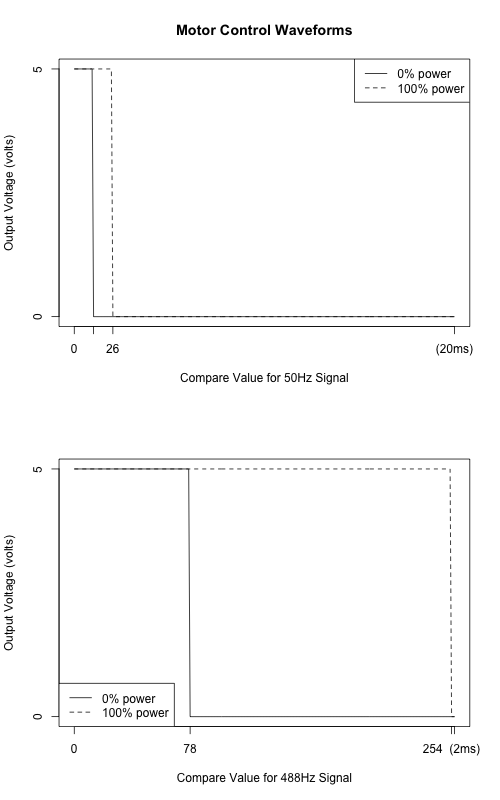
\includegraphics[scale=.65]{motorcontrolwaveforms}
\caption{Motor control signals for two different frequencies}
\end{center}
\end{figure}


